%%%%%%%%%%%%%%%%%%%%%%%%%%%%%%%%%%%%%%%%%%%%%%%%%%%%%%%%%%%%%%%%
%
% nand.tex -- A 2-input NAND gate build up in CMOS
%
% (c)2021, J. op den Brouw <J.E.J.opdenBrouw@hhs.nl>
%
% This is a schematic of a 2-input NAND-gate build up in CMOS
% technology. The schematic is drawn in CircuiTikZ.
%
%%%%%%%%%%%%%%%%%%%%%%%%%%%%%%%%%%%%%%%%%%%%%%%%%%%%%%%%%%%%%%%%%


\documentclass{standalone}
\usepackage{charter}
\usepackage[european,betterproportions]{circuitikz}

% Invert circles for pmos are open
\ctikzset{tripoles/pmos style/emptycircle}
% Arrows in the source connection
\ctikzset{tripoles/mos style/arrows}

% Positive displacement of the x coordinate of
% the right top pMOS transistor. Must be positive!
\newcommand{\xdisplacement}{2}

\begin{document}

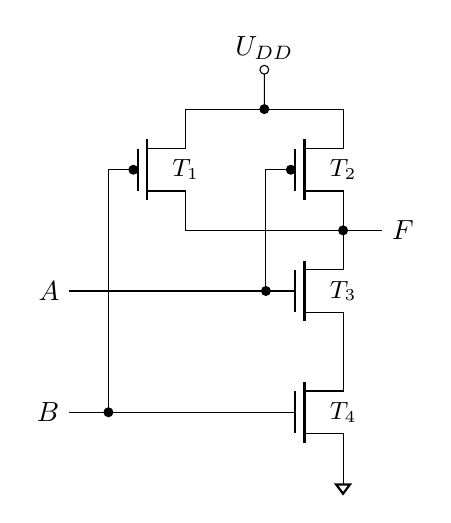
\begin{tikzpicture}

%% Place pMOS 1 and name it T1
\draw (0,0) node[pmos] (pmos1) {} node {\small $T_1$};
%% Place pMOS 2 and name it T2
\draw ($ (pmos1.S) + (\xdisplacement,0) $) node[pmos, anchor=S] (pmos2) {};
\node at ($ (pmos2.S)!.5!(pmos2.D) $) {\small $T_2$};

%% Draw short from sources pMOS1 to pMOS2
\draw (pmos1.S) to[short, -] (pmos2.S);
%% Draw from the middle of source pMOS1 and pMOS2: short up and place V_{DD}
\draw ($ (pmos1.S)!.5!(pmos2.S) $) to[short, *-o] ++(0,0.5) node[above] {$U_{DD}$};

%% Draw short from drain pMOS1 to pMOS2
\draw (pmos1.D) to[short, -*] (pmos2.D) to[short] ++(0.5,0) node[right] {$F$};
%%%%% Draw the output
%%%\draw (pmos2.D) to[short] ++(0.5,0) node[right] {$F$};

%% Place nMOS2 from drain of pMOS2 and name it T3
\draw (pmos2.D) node[nmos, anchor=D] (nmos2) {};
\node at ($ (nmos2.D)!.5!(nmos2.S) $) {\small $T_3$};
%% Place nMOS1 from source of nMOS1 and name it T4
\draw (nmos2.S) node[nmos, anchor=D] (nmos1) {};
\node at ($ (nmos1.D)!.5!(nmos1.S) $) {\small $T_4$};
%% Place ground from source of nMOS1
\draw (nmos1.S) node[sground,scale=.7] {};

%% Draw short from gate pMOS2 to gate nMOS2
\draw (pmos2.G) to[short, -*] (nmos2.G);

%% Draw a line from gate pMOS1 to gate connection of nMOS1
\draw (pmos1.G) to [short, -*] (pmos1.G |- nmos1.G);

%% Draw gate connections of gates nmos1 and nmos2
\draw (nmos2.G) -- ($ (pmos1.G |- nmos2.G) - (0.5,0) $) node[left] {$A$};
\draw (nmos1.G) -- ($ (pmos1.G |- nmos1.G) - (0.5,0) $) node[left] {$B$};

\end{tikzpicture}


\end{document}